%! Author = gbueno
%! Date = 22/07/2022

% Preamble
\documentclass[11pt]{article}

% Packages
\usepackage{amsmath}
\usepackage{ragged2e}
\usepackage{amsfonts}
\usepackage{hyperref}
\usepackage{stmaryrd}
\usepackage{wasysym}
\usepackage{graphicx}
\usepackage{multirow}
\usepackage[T1]{fontenc}

% Document
\begin{document}

    % Title
    \LARGE
    \centering
    RESUMO\\

    \Large
    Kirszenberg, A., Tochon, G., Puybareau, É., e Angulo, J. (2021). \textbf{Going beyond p-convolutions to learn grayscale morphological operator}\\
    \vspace{0.5cm}

    % Authory
    \normalsize
    \centering
    Autor: Guilherme Bueno Martins\\
    22 de julho de 2022\\
    \vspace{1cm}

    % Body
    \justifying


    \section{Introdução}
    \label{sec:introducao}

    Nos últimos anos houve um aumento de interesse na integração de operações morfológicas na estrutura de redes neurais devido a similiaridade existente entre operações morfologicas e de convolução.
Por conseguinte, emerge-se duas grandes linhas de pesquisa.
A primeira, que retoma ao final dos anos 80, substui operações da unidade \emph{perceptron}, como a multiplicação e soma pela adição e máximo, partindo de uma unidade \emph{perceptron} linear aos chamados \emph{perceptons} morfológicos não lineares.
A segunda explora a integração de operações morfológicas elementares nas Redes Neurias Convolucionais para a aprendizagem automática de seus pesos e formas ideais, tendo como maior problema as operações $\max$ e $\min$ como não deriváveis.

Uma primeira solução alternativa é o uso de aproximações diferenciáveis suaves para os tornar adaptáveis à abordagem de aprendizem do gradiente descendente convencional por meio da retropropagação.
Então, chama-se a atenção para as camadas p-convoluções (\emph{PConv}) pelos resutados promissores.
Baseando na estrutura da média contra-harmônica (CHM), pretende-se apresentar duas extensões para a camada \emph{PConv} com o interesse de implementa-los em arquiteturas de redes neurais profundas.


    \section{P-convolução: definição, propriedades e armadilhas}
    \label{sec:p-convolucao:-definicao-propriedades-e-armadilhas}

    Nesta seção, são detalhadas noções da p-convolução.

\subsection{Morfologia matemática em tons de cinza}
\label{subsec:morfologia-matematica-em-tons-de-cinza}

Em morfologia matemática, classicamente, uma imagem $f$ é representada como uma função 2D.
Defini-se $f: E \rightarrow \mathbb{R}$ com $x \in E$ sendo as coordenadas do píxel em um grid $E \subset \mathbb{Z}^{2}$ e os valores dos píxeis representados por $f(x) \in \mathbb{R}$.
Na morfologia matematática em tons de ciza, ambas a imagem $f$ e o elemento estruturante $b$ são valores reais (e não binário).
Ou seja, $b(x) \in \mathbb{R}$ e as operações de erosão $f \ominus b$ e dilatação $f \oplus b$ podem ser escrita como:

% Equation 1
\begin{equation}
(f \ominus b)(x)
    = \inf_{y \in E}\Big{\{} f(y) - b(x - y)\Big{\}}
    \label{eq:equation}
\end{equation}

% Equation 2
\begin{equation}
(f \oplus b)(x)
    = \sup_{y \in E}\Big{\{} f(y) + b(x - y)\Big{\}}
    \label{eq:equation2}
\end{equation}

O formualismo acima também é aplicável no uso de elementos estruturantes planos (binários) com

% Equation 3
\begin{equation}
    b(x) = \begin{cases}
               0        & \text{se } x \in B,       \\
               -\infty  & \text{caso contrário}     \\
    \end{cases}
    \label{eq:equation3}
\end{equation}
\\
onde $B \subset E$ é o suporte da função estruturante $b$.

\subsection{A média contra-harmônica e a p-convolução}
\label{subsec:a-media-contra-harmonica-e-a-p-convolucao}

A média ponderada de Lehmer, também conhecida como média contra-harmônica, é dada por um vetor não negativo $x = (x_{1}, x_{2}, \dots, x_{n}) \in (\mathbb{R}^{+})^{n}$, pesos não negativos $w = (w_{1}, w_{2}, \dots, w_{n}) \in (\mathbb{R}^{+})^{n}$ e com $p \in \mathbb{R}$.
Denotada por $CHM(x, w, p)$, é definida como:

% Equation 4
\begin{equation}
    CHM(x, w, p) = \frac{\sum_{i = 1}^{n} w_{i}x_{i}^{p}}{\sum_{i = 1}^{n} w_{i}x_{i}^{p-1}}
    \label{eq:equation4}
\end{equation}

Dentre os casos especiais, tem-se que $\lim_{p \to -\infty} CHM(x, w, p)$ é o mínimo dos elementos de x (ou seja, $\inf\{x_{i}\}$), bem como $\lim_{p \to +\infty} CHM(x, w, p)$ é o máximo dos elementos de x (ou, $\sup\{x_{i}\}$).

A p-convolução de uma imagem $f$ no píxel $x$ para valores do \emph{kernel} de convolução $w: W \subset E \to \mathbb{R}^{+}$ é definida como:

% Equation 5
\begin{equation}
    \begin{split}
        PConv(f, w, p)(x) = (f *_{p} w)(x) = \frac{(f^{p+1}*w)(x)}{(f^{p}*w)(x)} = \\
        = \frac{\sum_{y \in W(x)} f^{p+1}(y)w(x - y)}{\sum_{y \in W(x)} f^{p}(y)w(x - y)}
    \end{split}
    \label{eq:equation5}
\end{equation}
\\
onde $f^{p}(x)$ denota $(f(x))^{p}$ e, $W(x)$ é o suporte espacial do \emph{kernel} $w$ centrado em $x$.
Valendo-se das propriedades presentes na CHM, um comportamento morfológico é observado apartir de $p$.
Mais precisamente, uma pseudo-dilatação de $p \geq 0$ é alcançada quando $p \to +\infty$, bem como uma pseudo-erosão $p \leq 0$ para $p \to -\infty$.
Há, então, uma dominância do maior valor de píxel na vizinhança $W(x)$ para o píxel $x$ quando em uma dilatação (ou, em uma erosão, do menor valor de píxel na vizinha $W(x)$ para o píxel $x$) em uma soma ponderada.
Assintoticamente, $PConv(f, w, p)$ atua como uma diltação em tons de cinza não plana (ou como uma erosão em tons de cinza não plana) com função estruturante $b(x) = \frac{1}{p}\log(w(x))$:

% Equation 6
\begin{equation}
    \lim_{p \to +\infty} (f *_{p} w)(x) =
    \sup_{y \in W(x)} \Big{\{}f(y) + \frac{1}{p}\log(x(x - y))\Big{\}}
    \label{eq:equation6}
\end{equation}

% Equation 7
\begin{equation}
    \lim_{p \to -\infty} (f *_{p} w)(x) =
    \inf_{y \in W(x)} \Big{\{}f(y) - \frac{1}{p}\log(x(x - y))\Big{\}}
    \label{eq:equation7}
\end{equation}

De forma impírica, a aplicação das equações ~\ref{eq:equation6} e ~\ref{eq:equation7} são verdadeiras para $|p| > 10$.
Pode-se obter funções estruturantes planas usando pesos constantes nos \emph{kernels} de forma a satisfazer

% Equation 8
\begin{equation}
    w(x) = \begin{cases}
               1    & \text{, se } x \in W,                         \\
               0    & \text{, se } x \notin W \text{ e } |p| \geq 0 \\
    \end{cases}
    \label{eq:equation8}
\end{equation}
\\
e considerando, obviamente as limitações da definição de logaritmo.
Ou seja, quando $w(x) = 0$, temos as equações ~\ref{eq:equation6} e ~\ref{eq:equation7} como indefinidas.
Contudo, sendo a operação \emph{PConv} diferenciável, é compatível com a abordagem de aprendizagem via retropropagação com gradiente descendente.


\subsection{Limites da camada de p-convolução}
\label{subsec:limites-da-camada-de-p-convolucao}

Para que a \emph{PConv} seja definida em todas as suas entradas, são necessários que seus parâmetros $f$ e $w$ sejam estritamente positivos, além de outras limitações que devem ser evitadas.
São elas:

\begin{itemize}
    \item Se $w(x)$ ou $f^{p}(x)$ conter valores nulos, $\frac{1}{(f*_{p}w)(x)}$ não é definida;
    \item Se $f(x)$ contém valores nulos e $p$ é negativo, então $f^{p}(x)$ não é definida;
    e
    \item Se $f(x)$ conter valores negativos e $p$ diferir de nulo, tal que $p \notin \mathbb{R}$, $f^{p}(x)$ pode pertencer aos números complexos.
\end{itemize}

De forma geral, o cáculo a seguir é bastante utilizado para re-escalar valores de entrada no intervalo $[0, 1]$:

%Equation 9
\begin{equation}
    \text{maxmin}(f(x)) = \frac{f(x) - \min_{x \in E}f(x)}{\max_{x \in E}f(x) - \min_{x \in E}f(x)}.
    \label{eq:equation9}
\end{equation}

Sendo necessário re-escalar parâmetros de entrada entre camadas \emph{PConv} para se atingir uma pseudo-abertura ou pseudo-fechamento, por exemplo, aplica-se $1.0 + \text{maxmin}(f(x))$ de modo que a re-escala compreenda o intervalo $[1, 2]$.
Para se aplicar a re-escala, calcula-se:

% Equation 10
\begin{equation}
    f_{r}(x) = 1.0 + \text{maxmin}(f(x)) =
    1.0 + \frac{f(x) - \min_{x \in E}f(x)}{\max_{x \in E}f(x) - \min_{x \in E}f(x)}.
    \label{eq:equation10}
\end{equation}





    \section{Camadas $\mathcal{L}$Morph e $\mathcal{S}$Morph propostas}
    \label{sec:camadas-lmorph-e-smorph-propostas}

    Como exposto na subseção anterior~\ref{subsec:limites-da-camada-de-p-convolucao}, a camada \emph{PConv} possui alguns casos de desvantagens.
E, propõe-se duas novas camadas morfológicas baseadas nos princípios fundamentais da \emph{PConv} para fazê-las compatíveis com a morfologia matemática de tons de cinza geral.

\subsection{Apresentando à operação $\mathcal{L}$Morph}
\label{subsec:introduzindo-a-operacao-lmorph}

Com objetivo de contornar as funções não diferenciáveis $\min$ e $\max$ substituindo por aproximações diferenciáveis e suáveis, propõe-se a definição de $\mathcal{L}$Morph, inspirada na morfologia baseada na média de Lehmer.
Explorando o comportamento morfológico apresentado da camada $PConv$, apresenta-se:

% Equation 11
\begin{equation}
    \mathcal{L}\text{Morph}(f, w, p)(x) =
    \frac{\sum_{y \in W(x)} \big{(}f(y)w(x-y)\big{)}^{p+1}}{\sum_{y \in W(x)} \big{(}f(y)w(x-y)\big{)}^{p}}
    \label{eq:equation11}
\end{equation}
\\
onde $w: W \to \mathbb{R}^{+}$ é a função estruturante e $p \in \mathbb{R}$.
Interpretando a equação~\ref{eq:equation11} em relação a equação~\ref{eq:equation5} como $f(y) = f(y)w(x-y)$ e $1$ substituindo os valores de $w$ para que, de forma assintótica, reproduza-se o comportamento

% Equation 12
\begin{equation}
    \lim_{p \to +\infty} \mathcal{L}\text{Morph}(f, w, p)(x) =
    \sup_{y \in E}\Big{\{} f(y) + b(x - y)\Big{\}} = (f \oplus w)(x)
    \label{eq:equation12}
\end{equation}

% Equation 13
\begin{equation}
    \lim_{p \to +\infty} \mathcal{L}\text{Morph}(f, w, p)(x) =
    \inf_{y \in E}\Big{\{} f(y) + b(x - y)\Big{\}} = (f \ominus -w)(x)
    \label{eq:equation13}
\end{equation}

Pela mudança de sinal de $p$ é pode atingir uma pseudo-dilatação ou pseudo-erosão quando, respectivamente, $p > 0$ e $p < 0$.
Na prática, tal efeito é alcançado quando $|p| > 20$.

\begin{figure}[h]
    \caption{Linha superior: imagem de entrada, elemento estruturante não plano, dilatação alvo, erosão alvo. Linha média: pseudo-dilatação de $\mathcal{L}$Morph por incremento do valor de $p$. Linha inferior: pseudo-erosão de $\mathcal{L}$Morph por decremento do valor de $p$.}
    \centering
    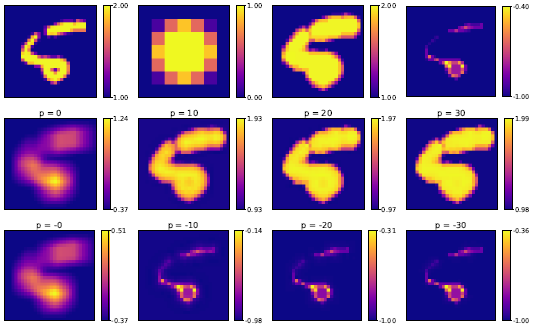
\includegraphics[scale=0.9]{images/LMorph}
    \label{fig:lmporh}
\end{figure}

Ressalta-se que as limitações de CHM são compartilhadas com $\mathcal{L}$Morph e que, por isso, a pseudo-erosão demonstrada na equação~\ref{eq:equation13} possui o elemento estruturante $w$ negativo.
Decorre-se que $\big{(}f(y)w(x-y)\big{)}$ tem as limitações de $f(x)$ citadas na seção~\ref{subsec:limites-da-camada-de-p-convolucao}, além da necessidade de reescalonamento.

\subsection{Introdução a operação $\mathcal{S}$Morph}
\label{subsec:introducao-a-operacao-smorph}

A função \emph{softmax} leva como entrada um vetor $x$ de $n$ números reais e os normaliza dentro de uma distribuição de probabilidade proporcional aos exponenciais dos números de entrada.
Alguns componentes do vetor $x$ podem ser negativos, ou maiores que $1$; e não totatlizar $1$.
Mas, após a aplicação da função, cada componente estará no intervalo $[0, 1]$ e resultarão $1$ quando somados.
A função \emph{softmax} $\mathcal{S}(x): \mathbb{R}^{n} \to [0, 1]^{n}$ é definida para $n > 1$ pela formula

% Equation 14
\begin{equation}
    \mathcal{S}(x_{i}) = \frac{e^{x_{i}}}{\sum_{j=1}^{n} e^{x_{j}}} \text{ para } i = 1, \dots, K
    \text{ e } x = (x_{i}, \dots, x_{n}) \in \mathbb{R}^{n}.
    \label{eq:equation14}
\end{equation}
\\
Ao invés de $e$, uma diferente base $b > 0$ pode ser usada.
Compete-se que se $0 > b > 1$, componentes de entrada menores resultarão em valores de sáida maiores.
Diminuir o valor de $b$ criará uma distribuição de probabilidade mais concentrada em torno das posições dos menores valores de entrada.
Por conseguinte, $b > 1$ resultará em valores de saídas maiores para os componentes de entrada maiores, e o aumento de $b$ implicará na concentração da distribuição de probabilidade em torno das posições dos maiores valores de entrada.
Escrevendo $b = e^{\alpha}$, temos a expressão

% Equation 15
\begin{equation}
    \mathcal{S}(x_{i}) = \frac{e^{\alpha x_{i}}}{\sum_{j=1}^{K} e^{\alpha x_{j}}}
    \label{eq:equation15}
\end{equation}

Para evitar as limitações da CHM, propõe-se a função $\alpha$-\emph{softmax} $S_{\alpha}(x)$ como uma aproximação definida por

% Equation 16
\begin{equation}
    \mathcal{S}_{\alpha}(x) = \frac{\sum_{i=1}^{n} x_{i}e^{\alpha x_{i}}}
    {\sum_{i=1}^{n} e^{\alpha x_{i}}}
    \label{eq:equation16}
\end{equation}
\\
para algum $x = (x_{1}, \dots, x_{n}) \in \mathbb{R}^{n}$ e $\alpha \in \mathbb{R}$.
A função em questão possui propriedades interessantes tais como $lim_{\alpha \to +\infty} \mathcal{S}_{\alpha}(x) = \max_{i}x_{i}$ e $lim_{\alpha \to -\infty} \mathcal{S}_{\alpha}(x) = \min_{i}x_{i}$ além de se beneficiar da falta da necessidade de reescalar suas entradas.
Explorando estas propriedades, defini-se a operação $\mathcal{S}$Morph (de \emph{Smooth Morphological} ou Morfologia Suave):

% Equation 17
\begin{equation}
    \mathcal{S}\text{Morph}(f, w, \alpha)(x) =
    \frac{\sum_{y \in W(x)} \big{(}f(y) + w(x - y)\big{)}e^{\alpha \big{(}f(y) + w(x - y)\big{)}}}
    {\sum_{y \in W(x)} e^{\alpha \big{(}f(y) + w(x - y)\big{)}}}
    \label{eq:equation17}
\end{equation}
\\
onde $w: W \to \mathbb{R}$ compre o papel de função estruturante, em que se pretende apartir da equação~\ref{eq:equation17} alcançar

% Equation 18
\begin{equation}
    \lim_{\alpha \to +\infty} = \mathcal{S}\text{Morph}(f, w, \alpha)(x) = (f \oplus w)(x)
    \label{eq:equation18}
\end{equation}

% Equation 19
\begin{equation}
    \lim_{\alpha \to -\infty} = \mathcal{S}\text{Morph}(f, w, \alpha)(x) = (f \ominus -w)(x)
    \label{eq:equation19}
\end{equation}

A capacidade de alternar entre as operações de pseudo-dilatação ou pseudo-erosão são definidas respectivamente por $alpha > 0$ e $alpha < 0$.

\begin{figure}[h]
    \caption{Linha superior: imagem de entrada, elemento estruturante não plano, dilatação alvo, erosão alvo. Linha média: pseudo-dilatação de $\mathcal{S}$Morph pelo incremento do valor de $\alpha$. Linha inferior: pseudo-erosão de $\mathcal{S}$Morph pelo decremento do valor de $\alpha$.}
    \centering
    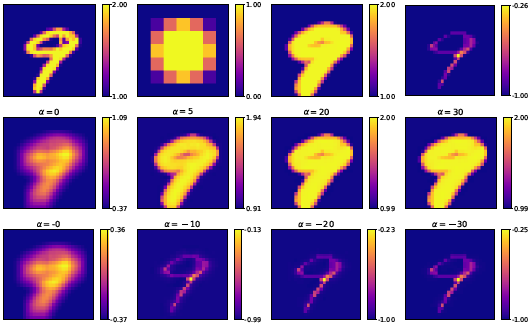
\includegraphics[scale=0.9]{images/SMorph}
    \label{fig:smorph}
\end{figure}



    \section{Experimentos conduzidos}
    \label{sec:experimentos-conduzidos}

    Esta seção apresenta o protocolo experimental e os resultados produzidos a partir deste protocolo.

\begin{figure}
    \caption{Elementos estruturante em tons de cinza alvos 7x7.}
    \centering
    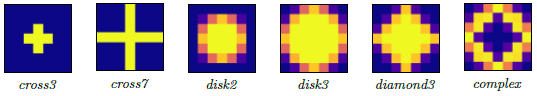
\includegraphics[scale=0.8]{images/ElementosEstruturantes}
    \label{fig:elementos-estruturantes}
\end{figure}

\subsection{Protocolo experimental}
\label{subsec:protocolo-experimental}

A seguir, foi avaliada a capacidade das camadas $\mathcal{L}$Morph e $\mathcal{S}$Morph propostas de aprenderem um elemento estruturante alvo e os resultados obtidos comparado com camada de \emph{PConv}.
Para tanto, as operações de dilatação $\oplus$, erosão $\ominus$, fechamento $\bullet$ e abertura $\circ$ foram aplicadas para todos os 60000 digitos do conjunto de dados MNIST, com elementos esturantes alvos apresentados na figura~\ref{fig:elementos-estruturantes}.
Mas precisamente, em se tratando das operaçãoes de dilatação e erosão, construi-se uma rede composta de apenas uma única camada seguida de um escalar/coeficiente linear de convolução 1x1x1 para re-escalar os valores de saída dentro do intervalor das imagens alvo.
Quanto as operações de fechamento e abertura, foram utilizados uma rede composta de duas camadas, respectivamente, dilatação e erosão e, erosão e dilatação.
Valendo salientar que, devidos as limitações já apresentadas, ambas as redes \emph{PConv} e $\mathcal{L}$Morph também tiveram que ser re-escaladas em [1, 2] antes de passarem por qualquer camada morfológica.
Todas as redes foram treinadas com um \emph{batch size} de 32, otimizado pela perda erro médio quadrático(MSE) com o otimizador Adam utilizando uma taxa de aprenizado $\eta = 0.01$.
A taxa de aprendizado do otimizador foi programada para decrementar por um fator de 10 quando o plato da perda se manter por 5 épocas consecutivas.
A convergence é tida como alcançada quando o plato da perda se estabilizar por 10 épocas consecutivas.

Para os filtros da camada \emph{PConv}, foram-se iniciados os filtros com $1$ e $p = 0$.
Para $\mathcal{L}$Morph, os filtros foram iniciados com distribuição normal dobrada com desvio padrão $\sigma = 0.01$ e $p = 0$.
Camadas $\mathcal{S}$Morph, com seus filtros inicializados com uma distribuição normal centrada com o desvio padrão $\sigma = 0.01$ e $\alpha = 0$.

Objetivando avaliar a desempenho das redes morfológicas para todos os cenários (isto é, para cada elemento estruturante operando $\oplus, \ominus, \bullet, \circ$), computou-se entre o filtro aprendido na convergência e o filtro alvo, a raiz do erro médio quadrático (RMSE).
Computando a perda na convergência bem como os valores dos parâmetros $p$ ou $\alpha$ úteis, também, como critério quanatitativo.

\begin{figure}
    \caption{Elementos estruturantes aprendidos (com seus correspondentes $p$ e $\alpha$ na convergência) pelas camadas \emph{PConv}, $\mathcal{L}$Morph e $\mathcal{S}$Morph em tarefas de dilatação $\oplus$ e erosão $\ominus$.}
    \centering
    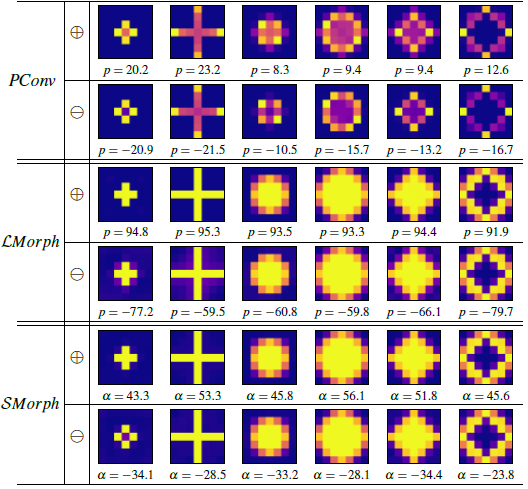
\includegraphics[scale=0.9]{images/ElementosEstrurantesAprendidos1}
    \label{fig:elementos-estruturantes-aprendidos-1}
\end{figure}

\begin{table}
    \caption{Perda do MSE na convergência e o RMSE entre o elemento estruturante aprendido apresentado pela figura~\ref{fig:elementos-estruturantes-aprendidos-1} e o alvo para as camadas \emph{PConv}, $\mathcal{L}$Morph e $\mathcal{S}$Morph nas tarefas de diltação $\oplus$ e erosão $\ominus$. Os melhores (menores) resultados estão em negrito.}
    \centering
    \label{tab:elementos-estruturantes-aprendidos-1}
    \resizebox{\textwidth}{!}{
        \begin{tabular}{*{10}l}
            &                            &      & \emph{cross3} & \emph{cross7} & \emph{disk2}  & \emph{disk3}  & \emph{diamond3} & \emph{complex} & \\
            \hline
            \multirow{4}{*}{\emph{PConv}}      & \multirow{2}{*}{$\oplus$}  & LOSS & 0.5           & 0.8           & 5.1           & 6.4           & 6.8 & 3.3 & $\times 10^{-4}$\\
            &                            & RMSE & 0.41          & 1.42          & 2.22          & 3.09          & 2.80            & 2.38           &                                          \\
            \cline{3-10}
            & \multirow{2}{*}{$\ominus$} & LOSS & 2.4           & 0.62          & 13            & 2.6           & 5.2             & 1.2            & $\times 10^{-5}$                         \\
            &                            & RMSE & 0.82          & 1.55          & 2.82          & 3.77          & 3.63            & 2.76           &                                          \\
            \hline
            \hline
            \multirow{4}{*}{$\mathcal{L}$Morh} & \multirow{2}{*}{$\oplus$}  & LOSS & 0.84          & 1.2           & 0.78          & 1.2 & 1.2 & 2.1 & $\times 10^{-5}$\\
            &                            & RMSE & \textbf{0.02} & \textbf{0.0 } & \textbf{0.02} & \textbf{0.05} & \textbf{0.01}   & \textbf{0.48} & \\
            \cline{3-10}
            & \multirow{2}{*}{$\ominus$} & LOSS & 1.1           & \textbf{0.37} & 1.3           & \textbf{0.37} & 0.58            & \textbf{1.1} & $\times 10^{-6}$ \\
            &                            & RMSE & \textbf{0.44} & 0.63          & 0.37          & 0.29          & 0.38            & \textbf{0.48}  &                                          \\
            \hline
            \hline
            \multirow{4}{*}{$\mathcal{S}$Morh} & \multirow{2}{*}{$\oplus$}  & LOSS & \textbf{1.8}  & \textbf{4.0} & \textbf{2.5} & \textbf{4.9} & \textbf{3.9} & \textbf{1.7} & $\times$ \textbf{10\textsuperscript{-7}} \\
            &                            & RMSE & 0.10          & 0.13          & 0.08          & 0.06          & 0.09            & 0.51           &                                          \\
            \cline{3-10}
            & \multirow{2}{*}{$\ominus$} & LOSS & 210           & 4.1           & \textbf{0.8}  & 4.1           & \textbf{4.3}    & \textbf{9.5} & $\times$ \textbf{10\textsuperscript{-7}} \\
            &                            & RMSE & 0.78          & \textbf{0.15} & \textbf{0.09} & \textbf{0.05} & \textbf{0.09}   & 0.51           &                                          \\
            \hline
        \end{tabular}
    }
\end{table}


\begin{figure}
    \caption{Elementos estruturantes aprendidos (com seus correspondentes $p$ e $\alpha$ na convergência) pelas camadas \emph{PConv}, $\mathcal{L}$Morph e $\mathcal{S}$Morph em tarefas de fechamento $\bullet$ e abertura $\circ$.}
    \centering
    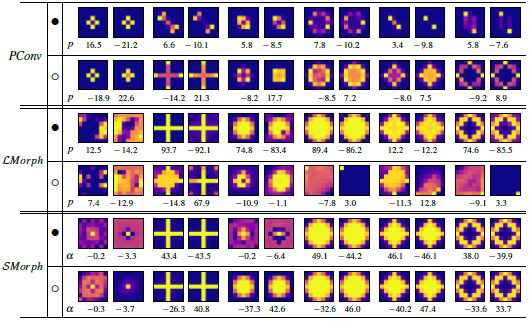
\includegraphics[scale=0.9]{images/ElementosEstrurantesAprendidos2}
    \label{fig:elementos-estruturantes-aprendidos-2}
\end{figure}

\begin{table}
    \caption{Perda do MSE na convergência e o RMSE entre o elemento estruturante aprendido apresentado pela figura~\ref{fig:elementos-estruturantes-aprendidos-2} e o alvo para as camadas \emph{PConv}, $\mathcal{L}$Morph e $\mathcal{S}$Morph nas tarefas de fechamento $\bullet$ e abertura $\circ$. Os melhores (menores) resultados estão em negrito.}
    \centering
    \label{tab:elementos-estruturantes-aprendidos-2}
    \resizebox{\textwidth}{!}{
        \begin{tabular}{*{10}l}
            &                            &      & \emph{cross3}                 & \emph{cross7}                 & \emph{disk2}                  & \emph{disk3}                  & \emph{diamond3}               & \emph{complex} & \\
            \hline
            \multirow{4}{*}{\emph{PConv}}      & \multirow{2}{*}{$\bullet$} & LOSS & 0.09                          & 5.1                           & 1.7                           & 1.0                           & 5.4 & 4.9 & $\times 10^{-e}$\\
            &                            & RMSE & \textbf{0.83} | \textbf{0.81} & 3.94 | 3.97                   & 2.82 | 3.07                   & 4.44 | 4.64                   & 4.34 | 4.61 & 3.68 | 3.65 &                  \\
            \cline{3-10}
            & \multirow{2}{*}{$\circ$}   & LOSS & \textbf{0.86}                 & 0.76                          & 4.8                           & 3.9                           & 4.4                           & 2.3                           & $\times 10^{-4}$                         \\
            &                            & RMSE & \textbf{0.91} | \textbf{0.32} & 1.45 | 0.87                   & 2.70 | 2.49                   & 3.10 | 2.52                   & 3.15 | 2.43 & 2.10 | 2.08 &                  \\
            \hline
            \hline
            \multirow{4}{*}{$\mathcal{L}$Morh} & \multirow{2}{*}{$\bullet$} & LOSS & \textbf{0.5}                  & 0.13 & \textbf{2.0} & 0.18 & 6.2 & 0.14 & $\times 10^{-4}$\\
            &                            & RMSE & 3.58 | 5.12                   & \textbf{0.01} | 0.63          & \textbf{0.14} | \textbf{1.16} & \textbf{0.07} | 0.40 & 0.75 | 0.95 & \textbf{0.47} | 0.99 & \\
            \cline{3-10}
            & \multirow{2}{*}{$\circ$}   & LOSS & 8.7                           & 36                            & 2.0                           & 2.7                           & 4.6                           & 2.5                           & $\times 10^{-3}$                         \\
            &                            & RMSE & 3.17 | 4.74                   & 2.90 | 1.20                   & 1.99 | 1.61                   & 2.81 | 5.56                   & 1.66 | 3.54                   & 2.72 | 3.98                   &                                          \\
            \hline
            \hline
            \multirow{4}{*}{$\mathcal{S}$Morh} & \multirow{2}{*}{$\bullet$} & LOSS & 1700                          & \textbf{0.31} & 4400 & \textbf{0.42} & \textbf{0.37} & \textbf{0.17} & $\times$ \textbf{10\textsuperscript{-6}} \\
            &                            & RMSE & 2.10 | 3.59                   & 0.14 | 0.08                   & 2.78 | 3.68                   & 0.08 | 0.01                   & 0.08 | 0.10                   & 0.52 | 0.52                   &                                          \\
            \cline{3-10}
            & \multirow{2}{*}{$\circ$}   & LOSS & 4700                          & \textbf{0.14}                 & \textbf{0.22}                 & \textbf{0.25}                 & \textbf{0.24} & \textbf{0.09} & $\times$ \textbf{10\textsuperscript{-6}} \\
            &                            & RMSE & 3.40 | 1.63                   & \textbf{0.18} | \textbf{0.02} & \textbf{0.05} | \textbf{0.01} & \textbf{0.02} | \textbf{0.02} & \textbf{0.02} | \textbf{0.01}  & \textbf{0.51} | \textbf{0.52} & \\
            \hline

        \end{tabular}
    }
\end{table}

\subsection{Resultados obtidos}
\label{subsec:resultados-obtidos}

Todas as redes (\emph{PConv}, $\mathcal{L}$Morph, $\mathcal{S}$Morph) conseguiram, por meio dos sinais dos parâmetros aplicar operações morfológicas corretamente.
A partir da magnetude observada na convergência, também é possível constatar que as operações aplicadas pelas redes podem ser consideradas dilatação e erosão (e, não simplesmente uma pseudo-dilatação ou pseudo-erosão).
Entretanto, enquanto o formato dos elementos estruturantes aprendidos pela camada de \emph{PConv} sofre um efeito de concavidade, as camadas $\mathcal{L}$Morph e $\mathcal{S}$Morph precisamente recuperam seus elementos estruturantes alvos.
Confirmados pelos valores de RMSE calculados entre o elemento estruturante alcançado durante a convergência e o elemento estruturante alvo apresentado na figura~\ref{fig:elementos-estruturantes}.
Mais precisamente, a operação de dilatação atingiu valores de RMSE mais baixos nas camadas de $\mathcal{L}$Morph e a erosão, com valores baixos nas camadas de $\mathcal{S}$Morph.
A figura \{\emph{incluir a figura 5}\} apresenta os elementos estruturantes aprendidos nas camadas de \emph{PConv}, $\mathcal{L}$Morph e $\mathcal{S}$Morph para as operações de abertura e fechamento.
Mas, desta vez, englobando duas camadas com filtros independentes um do outro.
A rede $\mathcal{L}$Morph foi capaz de aprender corretamente a operação e forma para os grandes elementos estruturantes nas operações de fechamento, com exceção do \emph{cross3} e \emph{disk2}.
Mas o contra-desempenho contantentemente falho percebido nas operações de abertura não até agora não foram explicados.
Tendo a rede $\mathcal{S}$Morph apresentado resultados pouco satisfatórios a pequenos elementos estruturantes para ambas operações de fechamento e abertura, é visto bons resultados nos maiores.
Nos casos extremos de pequenos elementos estruturantes alvos poderia vir da escala/convolução de coeficiênte linear 1x1x1, que super-compensa erros durante a fase de aprendizagem.
Poderia não ter aprendido corretamente todos os filtros por trás da escala//convolução de coeficiênte linear 1x1x1 com parametros $p$ e $\alpha$ não convergindo sobre os domínios de sinais corretos.





    \section{Conclusão}
    \label{sec:conclusao}

    Apresentadas as camadas morfológicas $\mathcal{L}$Morph e $\mathcal{S}$Morph inspiradas na camada \emph{PConv}, anteriormente baseadas nas propriedades do CHM visando atingir operações de dilatação e erosção em tons de cinza, foram aplicadas no conjunto de dados MNIST, 6 elementos estruturantes alvos de variados tamanhos e formas, para se avaliar o desempenho dessas camadas morfológicas de recuperar estes elementos estruturantes nas operações de dilatação, erosão, fechamento e abertura por meio treinamento.
No entanto, $\mathcal{S}$Morph baseado na função $\alpha$-softmax para os mesmos fins, sem as limitações encontradas em $\mathcal{L}$Morph e, consequentimente, \emph{PConv}, demonstrou resultados qualitativos e quantitativos melhores que os demais.

Os futuros trabalhos incluem investigação dos casos extremos das camadas bem como a integração destas a arquitetura de redes mais complexas e avaliações das mesmas em aplicações de processamento de imagens.

\end{document}